% coding: utf-8
\documentclass [a4paper,abstracton,titlepage]{scrartcl}
\pagestyle{plain}
\usepackage{makeidx}
\usepackage[table]{xcolor}
\usepackage{color}
\definecolor{LinkColor}{rgb}{0.33,0.42,0.18}
\definecolor{TableEvenColor}{rgb}{0.93,1,0.8}
\definecolor{TableOddColor}{rgb}{0.93,1,1}
\definecolor{TableBorderColor}{rgb}{0.55,0.67,0.73}
\definecolor{ListingBorderColor}{rgb}{0.55,0.55,0.55}
\definecolor{ListingBackgroundColor}{rgb}{0.95,0.95,0.95}
\definecolor{SidebarBorderColor}{rgb}{0.95,0.95,0.95}
\definecolor{SidebarBackgroundColor}{rgb}{1,1,0.93}
\usepackage{type1ec}
\usepackage[english]{babel}
\usepackage[
    pdftex,
    pdftitle={Report Interessent ZGV},
    pdfauthor={FH Technikum Wien},
    backref,
    pagebackref,
    breaklinks=true,
    unicode
    ]
    {hyperref}
\usepackage{enumerate}
\usepackage{graphicx}
\usepackage{longtable}
\usepackage[T1]{fontenc}
\usepackage{ucs}
\usepackage[utf8x]{inputenc}
\usepackage{textcomp}
\usepackage{alltt}
%\usepackage{listings}
\usepackage{verbatim}
\usepackage{moreverb}
\usepackage{upquote}

%\lstset{basicstyle=\footnotesize\ttfamily,showstringspaces=false,breaklines,frame=single, rulecolor=\color{ListingBorderColor}, xleftmargin=0cm, linewidth=0.95\textwidth}

 \setlength{\parskip}{1ex plus 0.5ex minus 0.2ex}

\makeatletter
\DeclareRobustCommand*\textsubscript[1]{%
  \@textsubscript{\selectfont#1}}
\def\@textsubscript#1{%
  {\m@th\ensuremath{_{\mbox{\fontsize\sf@size\z@#1}}}}}
\makeatother

\title{Report Interessent ZGV}
\author{FH Technikum Wien, \href{mailto:&lt;office@technikum-wien.at&gt;}{&lt;office@technikum-wien.at&gt;}}
\date{21.04.2015}
\publishers{\begin{tabular}{ll} \textbf{Revision:} & 1.0 \\    \end{tabular}}

\makeindex

\begin{document}

%\newcommand{texttesh}{textteshlig\/}

\label{header}\hypertarget{header}{}
\maketitle
\hypertarget{_studierende_interessent_mit_ohne_zgv_ausstellungsstaat_in_ausland}{}
\section{Studierende: Interessent mit/ohne ZGV-Ausstellungsstaat In-/Ausland}
\label{_studierende_interessent_mit_ohne_zgv_ausstellungsstaat_in_ausland}
\hypertarget{_beschreibung}{}
\subsection{Beschreibung}
\label{_beschreibung}
 \par\noindent{}Dieser Report liefert Kennzahlen zu Interessenten mit Zugangsvorraussetzungen welche im Ausland erworben wurden.
  \begin{description}
\item[%
\textbf{Attribute und Spalten}
]
  \begin{itemize}
\item%
Studienjahr

\item%
Gesamt: Gesamtzahl der Interessenten welche sich f\&{}uuml;r das entsprechende Studienjahr interessieren. Interessenten, welche sich f\&{}uuml;r mehrere Studieng\&{}auml;nge interessieren werden nur einmal gez\&{}auml;hlt.

\item%
Inland: Ausstellungsstaat der ZGV ist \&{}Ouml;sterreich.

\item%
Ausland: Ausstellungsstaat der ZGV ist ungleich \&{}Ouml;sterreich

\item%
KeineZGV: Ausstellungsstaat der ZGV ist nicht erfasst.

\item%
xStg Ausland: Anzahl der Interessenten mit ausl\&{}auml;ndischer ZGV welche sich f\&{}uuml;r x Studieng\&{}auml;nge interessieren.

\item%
xStg Inland: Anzahl der Interessenten mit \&{}ouml;sterr. ZGV welche sich f\&{}uuml;r x Studieng\&{}auml;nge interessieren.

\end{itemize}
\end{description}
\hypertarget{_inhalt}{}
\section{Inhalt}
\label{_inhalt}
\hypertarget{_chart}{}
\subsection{Chart}
\label{_chart}
 \par\noindent{}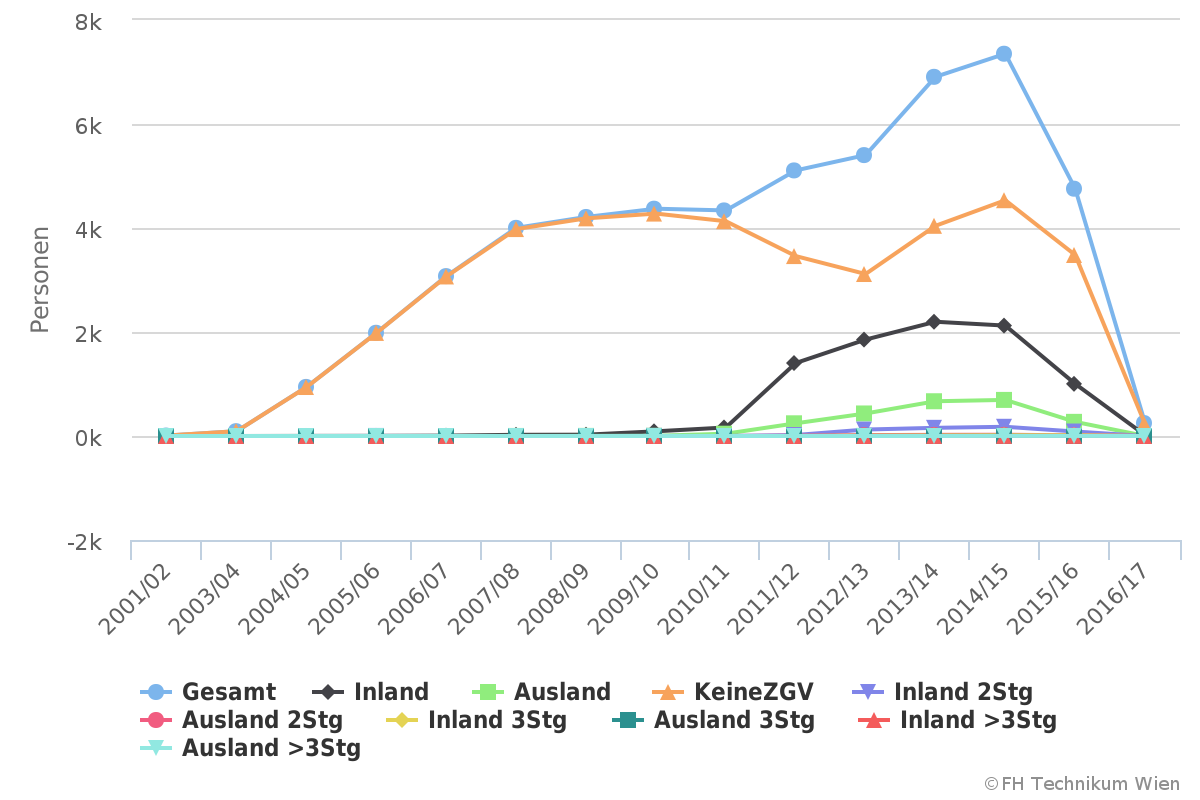
\includegraphics[]{images/chart6.png}
\hypertarget{_daten}{}
\subsection{Daten}
\label{_daten}
  \par\noindent
 \begin{tabular}{lllllllllllllll
 }
 
{\bfseries{}Studienjahr} &
{\bfseries{}Gesamt} &
{\bfseries{}Inland} &
{\bfseries{}Ausland} &
{\bfseries{}KeineZGV} &
{\bfseries{}Inland 2Stg} &
{\bfseries{}Ausland 2Stg} &
{\bfseries{}Inland 3Stg} &
{\bfseries{}Ausland 3Stg} &
{\bfseries{}Inland \textgreater{}3Stg} &
{\bfseries{}Ausland \textgreater{}3Stg} 
 \tabularnewline
 
2001/02 &
9 &
0 &
0 &
9 &
0 &
0 &
0 &
0 &
0 &
0 %
 \tabularnewline

2003/04 &
93 &
0 &
0 &
93 &
0 &
0 &
0 &
0 &
0 &
0 %
 \tabularnewline

2004/05 &
944 &
2 &
0 &
942 &
0 &
0 &
0 &
0 &
0 &
0 %
 \tabularnewline

2005/06 &
1985 &
3 &
0 &
1982 &
1 &
0 &
0 &
0 &
0 &
0 %
 \tabularnewline

2006/07 &
3075 &
7 &
0 &
3068 &
0 &
0 &
0 &
0 &
0 &
0 %
 \tabularnewline

2007/08 &
4003 &
23 &
1 &
3979 &
0 &
0 &
0 &
0 &
0 &
0 %
 \tabularnewline

2008/09 &
4212 &
25 &
2 &
4185 &
0 &
0 &
0 &
0 &
0 &
0 %
 \tabularnewline

2009/10 &
4371 &
90 &
4 &
4277 &
2 &
0 &
0 &
0 &
0 &
0 %
 \tabularnewline

2010/11 &
4338 &
164 &
44 &
4130 &
0 &
0 &
0 &
0 &
0 &
0 %
 \tabularnewline

2011/12 &
5107 &
1403 &
244 &
3460 &
19 &
5 &
1 &
0 &
0 &
0 %
 \tabularnewline

2012/13 &
5402 &
1854 &
433 &
3115 &
124 &
17 &
7 &
1 &
0 &
0 %
 \tabularnewline

2013/14 &
6907 &
2197 &
668 &
4042 &
157 &
22 &
11 &
1 &
1 &
0 %
 \tabularnewline

2014/15 &
7351 &
2123 &
694 &
4534 &
177 &
24 &
16 &
2 &
2 &
1 %
 \tabularnewline

2015/16 &
4756 &
1003 &
272 &
3481 &
86 &
13 &
15 &
0 &
2 &
1 %
 \tabularnewline

2016/17 &
249 &
17 &
1 &
231 &
0 &
0 &
0 &
0 &
0 &
0 %
 \tabularnewline
 \end{tabular}
  \begin{description}
\item[%
\textbf{M\&{}ouml;gliche Fehlerquellen}
]
  \begin{itemize}
\item%
ZGV: Der Ausstellungsstaat der ZGV ist nicht gut gepflegt. Es kann daher vorkommen, dass zwar die Zugangsvoraussetzung gegeben ist, aber der Ausstellungsstaat fehlt und deshalb die Zahlen in dieser Auswertung etwas verschoben sind.

\item%
Ausstellungsstaat: Dieses Attribut wurde im WS2011 im Zuge einer neuen BIS-Verordnung eingef\&{}uuml;hrt. Die Zahlen vor dem WS2011 sind demnach mit gro\&{}szlig;er Wahrscheinlichkeit schlecht gepflegt.

\end{itemize}
\end{description}
\label{footer}\hypertarget{footer}{}
\end{document}
